\documentclass[mathserif]{beamer}

%\usepackage{graphicx}
\usepackage{amsmath,amssymb,amsthm, mathtools}
\usepackage{xcolor}
%\usepackage{bbold}
%\usepackage[skins]{tcolorbox}
%\newcommand{\ou}{\mathbb 1}
\newcommand{\<}{\langle}
\renewcommand{\>}{\rangle}
\newcommand{\supp}{\operatorname{supp}}
%\newcommand{\wit}{\operatorname{wit}}
\newcommand{\Tr}{\operatorname{tr}\,}
\newcommand{\Se}{\mathcal S}
\newcommand{\Ee}{\mathcal E}
\newcommand{\Fe}{\mathcal F}
\newcommand{\Me}{\mathcal M}
\newcommand{\Ne}{\mathcal N}
\newcommand{\Ce}{\mathcal C}
\newcommand{\Ha}{\mathcal H}
\newcommand{\Le}{\mathcal L}
\newcommand{\Ka}{\mathcal K}
\def\llangle{\langle\kern-0.4ex\langle}
\def\rrangle{\rangle\kern-0.4ex\rangle}
\def\doublek{\rrangle\kern-0.3ex\llangle}
\setbeamertemplate{itemize items}[circle]

\setbeamercolor{footnote mark}{fg=orange}
\setbeamercolor{footnote}{fg=brown}

\newcommand{\myfootnote}[1]{
    \renewcommand{\thefootnote}{}
    \footnotetext{\hspace{-16.5pt}\scriptsize#1}
    \renewcommand{\thefootnote}{\arabic{footnote}}
}

\setbeamertemplate{section page}
{
    \begin{centering}
    \begin{beamercolorbox}[sep=12pt]{part title}
    \usebeamerfont{section title}\insertsection\par
    \end{beamercolorbox}
    \end{centering}
}

%\newtcolorbox{mybox}[1][]{before skip=3mm, after skip=3mm, enhanced,colbacktitle=blue!10!white, coltitle=blue!50!black,colback=white,colframe=white!98!black,drop fuzzy shadow southeast={black!50!white}, #1}
%\newcommand{\vun}{\rotatebox[origin=c]{90}{$\subseteq$}}


%\newtcolorbox{mybox}[1][]{before skip=3mm, after skip=3mm, enhanced,colbacktitle=blue!10!white, coltitle=blue!50!black,colback=white,colframe=white!98!black,drop fuzzy shadow southeast={black!50!white}, #1}
%\newcommand{\vun}{\rotatebox[origin=c]{90}{$\subseteq$}}


%\titlegraphic{
\includegraphics[width=1.5cm]{logomu.pdf}\hspace*{4.75cm}~%
%   
\includegraphics[width=1.5cm]{logosav}}

\title{On $\alpha-z$-R\'enyi divergences in von Neumann algebras}
\subtitle{\small\color{black}based on: Fumio Hiai and AJ, arxiv:2404.07617}
\author{Anna Jen\v cov\'a}
\institute{Mathematical Institute, Slovak Academy of Sciences, Bratislava,
Slovakia\\[5mm]

\includegraphics[width=1.5cm]{logomu.pdf}\hspace*{4.75cm}~%
   
\includegraphics[width=1.5cm]{logosav}
}


%\titlegraphic{
\includegraphics[width=1.5cm]{logomu.pdf}\hspace*{4.75cm}~%
%   
\includegraphics[width=1.5cm]{logosav}
%}
\date{Towards Infinite Dimension and Beyond in Quantum Information, Granada, May 9, 2024}

\begin{document}
\begin{frame}
  \titlepage
\end{frame}


\begin{frame}{The $\alpha$-$z$-R\'enyi divergences}


For density operators $\rho$, $\sigma$ on a finite dimensional Hilbert space:
\[
D_{\alpha,z}(\rho\|\sigma)=\frac{1}{\alpha-1}\log
\frac{\mathrm{Tr}\bigl(\rho^{\frac{\alpha}{2z}}\sigma^{\frac{1-\alpha}{z}}
\rho^{\frac{\alpha}{2z}}\bigr)^z}{\mathrm{Tr}\,\rho},
\]
where $0<\alpha\ne 1$ and $z>0$.\myfootnote{V. Jaksi\'c et al, 2011}
\myfootnote{K. Audenaert, N. Datta, 2015}

\bigskip

For each $z>0$: a quantum extension of classical R\'enyi $\alpha$-divergences for
probability vectors $p,q$:
\[
D_\alpha(p\|q)=\frac{1}{\alpha}\log(\sum_i p_i^\alpha q_i^{1-\alpha}).
\]





\end{frame}

\begin{frame}{The $\alpha$-$z$-R\'enyi divergences}

Important special cases:

\medskip 

\begin{itemize}
\item \structure{Relative entropy}:
\[
\lim_{\alpha\to 1}D_{\alpha,z}(\rho\|\sigma)=D_1(\rho\|\sigma)=\frac{\mathrm{Tr}\bigl(\rho(\log \rho-\log \sigma)\bigr)}{\mathrm{Tr}\,\rho}
\]

\item \structure{Petz-type (standard) R\'enyi divergence}: $z=1$, $0<\alpha\ne 1$
\[
D_\alpha(\rho\|\sigma)=\frac{1}{\alpha-1}\log\frac{\mathrm{Tr}\bigl(\rho^{\alpha}\sigma^{1-\alpha}\bigr)}{\mathrm{Tr}\,\rho}
\]
\item \structure{Sandwiched R\'enyi divergence}:  $0<z=\alpha\ne 1$
\[
\tilde
D_\alpha(\rho\|\sigma)=\frac{1}{\alpha-1}\log\frac{\mathrm{Tr}\bigl(\sigma^{\frac{1-\alpha}{2\alpha}}\rho\sigma^{\frac{1-\alpha}{2\alpha}}\bigr)}{\mathrm{Tr}\,\rho}
\]


\end{itemize}




\end{frame}

\begin{frame}{Data processing inequality (DPI)}

For a quantum channel (CPTP map) $\Phi$ and any $\rho$, $\sigma$:
\[
D_{\alpha,z}(\Phi(\rho)\|\Phi(\sigma))\le D_{\alpha,z}(\rho\|\sigma)
\]
- not true for all values of $\alpha$, $z$:

\medskip


\begin{itemize}
\item Petz-type:\footnote{Ando's convexity theorem, 1979}  $\alpha\in (0,1)\cup (1,2]$;
\item sandwiched:\footnote{S. Beigi,
2013; Frank and Lieb, 2013}
 $\alpha\in [1/2,1)\cup (1,\infty]$;\item general case:\footnote{Carlen, Frank and Lieb,
 2018; Zhang, 2020}
\[
0 < \alpha < 1,\quad  \max\{\alpha, 1 - \alpha\} \le  z 
\]
or
\[
\alpha > 1,\quad  \max\{\alpha/2, \alpha - 1\} \le  z \le \alpha.
\]
\end{itemize}


\end{frame}

\begin{frame}{Outline of this talk}

\begin{itemize}
\item extension of $D_{\alpha,z}$ to the setting of \structure{von Neumann
algebras}

\item  DPI with respect to
\structure{positive} trace preserving maps (within the same bounds on parameters as in
finite dimensions)

\item equality in DPI implies \structure{sufficiency (reversibility)} for 2-positive
trace preserving maps

\end{itemize}

\medskip

Our tools
\medskip

\begin{itemize}
\item  variational formula for $D_{\alpha,z}$
\item known results in the sandwiched case
\item properties of conditional expectations

\end{itemize}


\end{frame}

\begin{frame}{von Neumann algebra extensions}

The R\'enyi divergences were defined for normal positive functionals $\psi,\varphi$ on a
von Neumann algebra, using some technical tools:

\medskip

\begin{itemize}
\item \structure{Araki relative entropy}\footnote{Araki, 1976}:  relative modular operator
$\Delta_{\psi,\varphi}$
\item Petz-type (\structure{Petz quasi divergence})\footnote{Petz, 1985}:
$\Delta_{\psi,\varphi}$
\item sandwiched R\'enyi divergence:\footnote{Berta, Scholtz and Tomamichel,
2018; AJ, 2018; 2021}
 Araki-Masuda or Kosaki $L^p$-spaces
\item general $\alpha$-$z$ R\'enyi divergences:\footnote{Kato and Ueda, 2023; Kato, 2024}
Haagerup $L^p$-spaces

 \end{itemize}


\end{frame}

\begin{frame}{von Neumann algebras and Haagerup $L^p$-spaces}


Let $\Me$ be a  von Neumann algebra $\Me$, with predual $\Me_*$.

\bigskip 

\begin{itemize}


\item Haagerup $L^p$-space $L^p(\Me)$, $0<p\le \infty$

\medskip

\item $\Me=L^\infty(\Me)$, $\Me_*\simeq L^1(\Me)$, $\varphi\mapsto h_\varphi$,
$\Tr(h_\varphi)=\varphi(1)$

\medskip

\item order isomorphism: $\Me_*^+\ni \varphi\mapsto h_\varphi \in L^1(\Me)^+$


\medskip

\item polar decomposition: for $0<p<\infty$,  $k\in L^p(\Me)$, $k=u|k|$:
\[
u\in \Me \text{ partial isometry},\  |k|=h_\varphi^{1/p}\in L^p(\Me)^+,\ \varphi\in
\Me_*^+
\]

\end{itemize}
\end{frame}

\begin{frame}{von Neumann algebras and Haagerup $L^p$-spaces}


For $0<p<\infty$, $k\in L^p(\Me)$,  put $\|k\|_p=(\Tr|k|^p)^{1/p}$.

\bigskip

\begin{itemize}


\item For $1<p<\infty$,  $\|k\|_p$ is a norm in $L^p(\Me)$, which  is a reflexive Banach space, 
with dual $L^p(\Me)^*\simeq L^q(\Me)$,
$1/p+1/q=1$ 

\medskip

\item $\|k\|_p$ is a quasi norm for $0<p<1$

\medskip 
\item H\"older inequality: for $1/p+1/q=1/r$, $0<p,q,r\le \infty$, $h\in L^p(\Me)$, $k\in
L^q(\Me)$:
\[
hk\in L^r(\Me) \ \text{ and }\ \|hk\|_r\le \|h\|_p\|k\|_q
\]

\end{itemize}

\end{frame}

\begin{frame}{$D_{\alpha,z}$ for von Neumann algebras}

Let $0<\alpha\ne1$, $0<z$. 
For $\psi,\varphi\in \Me_*^+$, $\psi\ne 0$,  we define\footnote{Kato and Ueda, 2023; Kato 2024}
\[
D_{\alpha,z}(\psi\|\varphi)=\frac{1}{\alpha-1}\log
\frac{Q_{\alpha,z}(\psi\|\varphi)}{\psi(1)}
\]
where
\[
Q_{\alpha,z}(\psi\|\varphi):=\begin{dcases} \Tr
\left(h_\varphi^{\frac{1-\alpha}{2z}}h_\psi^{\frac{\alpha}{z}}h_\varphi^{\frac{1-\alpha}{2z}}\right)^z, &
\text{if } 0<\alpha<1,\\[0.5em]
\|x\|_z^z, & \text{if } \alpha>1 \text{ and }
h_\psi^{\frac{\alpha}{z}}=h_\varphi^{\frac{\alpha-1}{2z}}xh_\varphi^{\frac{\alpha-1}{2z}}
\\[-0.1em] & \text{with } x\in s(\varphi)L^z(\Me)s(\varphi),\\[1em]
\infty,& \text{otherwise}.
\end{dcases}
\]


\end{frame}

\begin{frame}{Positive maps and the Petz dual}


Let $\Me,\Ne$ be von Neumann algebras, $\gamma:\Ne \to \Me$ positive unital normal map.

\medskip
\begin{itemize}
\item The \structure{predual map}: $\gamma_*: L^1(\Me)\to L^1(\Ne)$,
\[
 \gamma_*(h_\omega):=h_{\omega\circ\gamma},\quad \text{positive, trace
preserving}
\]
\item Let $\rho\in \Me_*^+$, $e:=s(\rho)$, $e_0:= s(\rho\circ \gamma)$.
The \structure{Petz dual} $\gamma^*_\rho:e\Me e\to e_0\Ne e_0$ is determined by
%\[
%h_{\rho\circ\gamma}^{1/2}\gamma_\rho^*(a)h_{\rho\circ\gamma}^{1/2}
%=\gamma_*\bigl(h_\rho^{1/2}ah_\rho^{1/2}\bigr),
%\qquad a\in e\Me e,
%\]
%equivalently,
\[
(\gamma^*_\rho)_*\bigl(h_{\rho\circ\gamma}^{1/2}bh_{\rho\circ\gamma}^{1/2}\bigr)
=h_\rho^{1/2}\gamma(b)h_\rho^{1/2},\qquad b\in\Ne^+.
\]
 - positive, unital and normal,

 - $n$-positive whenever $\gamma$ is.


\end{itemize}


\end{frame}

\begin{frame}{DPI in von Neumann algebra setting}

For any $\psi,\varphi\in \Me_*^+$, $\psi\ne 0$, and a positive unital normal map
$\gamma:\Ne\to \Me$:
\[
D_{\alpha,z}(\psi\circ\gamma\|\varphi\circ\gamma)\le D_{\alpha,z}(\psi\|\varphi).
\]

This was already proved for:

\medskip

\begin{itemize}
\item Petz type: $\alpha\in (0,1)\cup(1,2]$, $\gamma$ a Schwarz map\footnote{Petz, 1985},
\item sandwiched: $\alpha\in [1/2,1)\cup (1,\infty]$, $\gamma$ completely
positive\footnote{Berta, Scholz and Tomamichel, 2018}, $\gamma$ positive\footnote{AJ,
2018, 2021}
\item $D_{\alpha,z}$ with $0<\alpha<1$, $\max\{\alpha,1-\alpha\}\le z$, $\gamma$
positive\footnote{Kato, 2024}
\end{itemize}



\end{frame}

\begin{frame}{Variational expressions}

Let $\psi,\varphi\in \Me_*^+$, $\psi\ne 0$.\myfootnote{Finite dimensions: Zhang, 2020}
\begin{enumerate}
\item[(i)] Let $0<\alpha<1$, $\max\{\alpha,1-\alpha\}\le z$. Then
\begin{multline*}
Q_{\alpha,z}(\psi\|\varphi)=\inf_{a\in \Me^{++}}\left\{\alpha
\Tr\left(\left(h_\psi^{\frac{\alpha}{2z}}ah_\psi^{\frac{\alpha}{2z}}\right)^{\frac{z}{\alpha}}\right)\right. \\
\left.+(1-\alpha)
\Tr\left(\left(h_\varphi^{\frac{1-\alpha}{2z}}a^{-1}h_\varphi^{\frac{1-\alpha}{2z}}\right)^{\frac{z}{1-\alpha}}\right) \right\}.
\end{multline*}

\item[(ii)] Let $\alpha>1$, $\max\{\alpha/2,\alpha-1\}\le z$. Then
\begin{multline*}
Q_{\alpha,z}(\psi\|\varphi)=\sup_{a\in \Me^+} \left\{\alpha
\Tr\left(\left(h_\psi^{\frac{\alpha}{2z}}ah_\psi^{\frac{\alpha}{2z}}\right)^{\frac{z}{\alpha}}\right)\right.
\\ \left. -(\alpha-1)
\Tr\left(\left(h_\varphi^{\frac{\alpha-1}{2z}}ah_\varphi^{\frac{\alpha-1}{2z}}\right)^{\frac{z}{\alpha-1}}\right) \right\}.
\end{multline*}
\end{enumerate}


\end{frame}

\begin{frame}{Useful inequalities}

 $\gamma:\Ne\to \Me$  a normal positive unital map,  $\rho\in \Me_*^+$,  $b\in \Ne^+$. 

\bigskip
\begin{enumerate}
\item[(1)] If $p\in [1/2,1)$, then 
\[
\Big\|h_{\rho\circ\gamma}^{\frac{1}{2p}}bh_{\rho\circ\gamma}^{\frac{1}{2p}}\Big\|_p\le
\Big\|h_{\rho}^{\frac{1}{2p}}\gamma(b)h_{\rho}^{\frac{1}{2p}}\Big\|_p.
\]
\end{enumerate}

\begin{proof} Let $\omega\in \Ne_*^+$,
$h_\omega=h_{\rho\circ\gamma}^{\frac12}bh_{\rho\circ\gamma}^{\frac12}$.
\begin{align*}
\Big\|h_{\rho}^{\frac{1}{2p}}\gamma(b)h_{\rho}^{\frac{1}{2p}}\Big\|^p_p&=Q_{p,p}(\omega\circ
\gamma^*_\rho\|\rho)=Q_{p,p}(\omega\circ
\gamma^*_\rho\|\rho\circ\gamma\circ\gamma_\rho^*)\\
&\ge\footnotemark 
Q_{p,p}(\omega\|\rho\circ\gamma)=\Big\|h_{\rho\circ\gamma}^{\frac{1}{2p}}bh_{\rho\circ\gamma}^{\frac{1}{2p}}\Big\|^p_p
\end{align*}\footnotetext{Sandwiched case: AJ, 2021}



\end{proof}




\end{frame}

\begin{frame}{Useful inequalities}

 $\gamma:\Ne\to \Me$  a normal positive unital map,  $\rho\in \Me_*^+$,  $b\in \Ne^+$. 

\bigskip
\begin{enumerate}
\item[(2)] If $p\in [1,\infty]$, then 
\[
\Big\|h_{\rho\circ\gamma}^{\frac{1}{2p}}bh_{\rho\circ\gamma}^{\frac{1}{2p}}\Big\|_p\ge
\Big\|h_{\rho}^{\frac{1}{2p}}\gamma(b)h_{\rho}^{\frac{1}{2p}}\Big\|_p.
\]
\end{enumerate}

\begin{proof} Let $\omega\in \Ne_*^+$,
$h_\omega=h_{\rho\circ\gamma}^{\frac12}bh_{\rho\circ\gamma}^{\frac12}$.
\begin{align*}
\Big\|h_{\rho}^{\frac{1}{2p}}\gamma(b)h_{\rho}^{\frac{1}{2p}}\Big\|^p_p&=Q_{p,p}(\omega\circ
\gamma^*_\rho\|\rho)=Q_{p,p}(\omega\circ
\gamma^*_\rho\|\rho\circ\gamma\circ\gamma_\rho^*)\\
&\le\footnotemark 
Q_{p,p}(\omega\|\rho\circ\gamma)=\Big\|h_{\rho\circ\gamma}^{\frac{1}{2p}}bh_{\rho\circ\gamma}^{\frac{1}{2p}}\Big\|^p_p
\end{align*}\footnotetext{Sandwiched case: AJ, 2018}



\end{proof}

\end{frame}


\begin{frame}{DPI in the von Neumann algebra setting}

Let $\psi,\varphi\in \Me_*^+$, $\psi\ne 0$ and let $\gamma:\Ne\to \Me$ be a normal positive
unital map. 

\bigskip 

Assume either of the following conditions:
\medskip

\begin{enumerate}
\item[(i)] $0<\alpha<1$, $\max\{\alpha,1-\alpha\}\le z$,
\item[(ii)] $\alpha>1$, $\max\{\alpha/2,\alpha-1\}\le z\le \alpha$.
\end{enumerate}

\bigskip

Then we have
\[
D_{\alpha,z}(\psi\circ\gamma\|\varphi\circ\gamma)\le D_{\alpha,z}(\psi\|\varphi).
\]

\end{frame}

\begin{frame}{DPI in the von Neumann algebra setting}

Let $0<\alpha<1$, $\max\{\alpha,1-\alpha\}\le z$.  We have

\medskip 

\[
Q_{\alpha,z}(\psi\|\varphi)=\inf_{a\in \Me^{++}}\left\{\alpha
\Big\|h_\psi^{\frac{1}{2p}}ah_\psi^{\frac{1}{2p}}\Big\|_p^{p}
+(1-\alpha) \Big\|h_\varphi^{\frac{1}{2r}}a^{-1}h_\varphi^{\frac{1}{2r}}\Big\|_r^{r}
\right\},
\]
with $p:=\frac{z}{\alpha}$, $r:=\frac{z}{1-\alpha}$. In the above bounds, $p,r\ge 1$.

\bigskip

By the inequality \structure{(2)} and the Choi inequality:
\[
\gamma(b)^{-1}\le \gamma(b^{-1}),
\]
we get
\[
Q_{\alpha,z}(\psi\circ\gamma\|\varphi\circ\gamma)\ge Q_{\alpha,z}(\psi\|\varphi).
\]


\end{frame}



\begin{frame}{DPI in the von Neumann algebra setting}

Let $\alpha>1$, $\max\{\alpha/2,\alpha-1\}\le z\le \alpha$.  We have

\medskip 

\[
Q_{\alpha,z}(\psi\|\varphi)=\sup_{a\in \Me^{+}}\left\{\alpha
\Big\|h_\psi^{\frac{1}{2p}}ah_\psi^{\frac{1}{2p}}\Big\|_p^{p}
-(\alpha-1) \Big\|h_\varphi^{\frac{1}{2q}}ah_\varphi^{\frac{1}{2q}}\Big\|_q^{q}
\right\},
\]
with $p:=\frac{z}{\alpha}$, $q:=\frac{z}{\alpha-1}$. In the above bounds, $p\in [1/2,1)$,
$q\ge 1$.

\bigskip

By the inequalities \structure{(1)} and  \structure{(2)}
we get
\[
Q_{\alpha,z}(\psi\circ\gamma\|\varphi\circ\gamma)\le Q_{\alpha,z}(\psi\|\varphi).
\]

\end{frame}

\begin{frame}{Sufficient channels and equality in DPI}

A \structure{channel} is a 2-positive unital normal map $\gamma:\Ne\to \Me$.

\bigskip

Let $\psi,\varphi\in \Me_*^+$. We say that $\gamma$ is \structure{sufficient} with respect to
$\{\psi,\varphi\}$ if there exists a \structure{recovery channel} $\beta:\Me\to \Ne$ such that\myfootnote{Petz, 1986, 1988}
\[
\psi\circ \gamma\circ \beta=\psi,\qquad \varphi\circ \gamma\circ \beta=\varphi.
\]

\bigskip

\structure{Petz theorem}: Assume that $D_1(\psi\|\varphi)<\infty$. Then $\gamma$ is
sufficient with respect to $\{\psi,\varphi\}$ if and only if
\[
D_1(\psi\circ\gamma\|\varphi\circ\gamma)=D_1(\psi\|\varphi).
\]
A similar result holds for the transition probability ($D_{\frac12,1}$).






\end{frame}



\begin{frame}{Known results on equality in DPI}

Characterization of sufficient channels:

\bigskip

\begin{itemize}
\item Petz-type: $D_{\alpha,1}$, $\alpha\in (0,1)\cup (1,2)$\footnote{AJ and Petz, 2006;
Hiai et al, 2011; 
Hiai and Mosonyi 2017; Hiai, 2018}


\medskip

\item sandwiched: $D_{\alpha,\alpha}$, $\alpha\in (1/2,1)\cup\structure{(1,\infty)}$\footnote{AJ,
2018, 2021}

\end{itemize}

\bigskip

Other equality conditions for $D_{\alpha,z}$ were found in finite dimensions\footnote{Leditzky, Rouz\'e and
Datta, 2017;  Hiai and Mosonyi, 2017; Zhang 2020}
\medskip

- no clear relation to sufficiency of channels (apart from some special cases).


\end{frame}



\begin{frame}{Universal recovery channel}


The Petz dual $\gamma_\varphi^*$ is a \structure{universal recovery channel}:


Let $\psi\in \Me_*^+$ be such that  $s(\psi)\le s(\varphi)$. Then  $\gamma$ is sufficient with respect to $\{\psi,\varphi\}$ if and only if 
\[
\psi\circ \gamma\circ \gamma_\varphi^*=\psi.
\]
\medskip 




\end{frame}






\begin{frame}{Equality in DPI}

What are the conditions for
\[
D_{\alpha,z}(\psi\circ\gamma\|\varphi\circ \gamma)=D_{\alpha,z}(\psi\|\varphi)?
\]

If $\gamma$ is 2-positive, the equality is \alert{in some cases} equivalent to existence of a
\structure{recovery map}: 2-positive, unital, normal map $\beta:\Me\to \Ne$ such that
\[
\psi\circ \gamma\circ \beta=\psi,\qquad \varphi\circ \gamma\circ \beta=\varphi.
\]
$\equiv$  $\gamma$ is \structure{sufficient} with respect to
$\{\psi,\varphi\}$\footnote{Petz, 1986, 1988}.


\end{frame}


\begin{frame}{Equality in DPI and sufficiency}








\end{frame}



\end{document}
\begin{frame}{Quantum sufficiency}

Let $\Se$ be a family of quantum states, $\Phi$ a quantum channel.

\bigskip

Possible notions of sufficiency (equivalent in the classical case):
\medskip

\begin{enumerate}
\item[(a)] definitions based on \structure{conditional expectations} - too restrictive
\item[(b)] \structure{reversibility} of $\Phi$ on $\Se$
\item[(c)] preserving \structure{quantum divergences} (relative entropy, R\'enyi
divergences) %\hfill {\footnotesize\textcolor{orange}{(Kullback-Leibler, Csisz\' ar)}}
\item[(d)] preserving optimal errors in \structure{hypothesis testing} %\hfill {\footnotesize\textcolor{orange}{(Pfanzagl)}}
\end{enumerate}

\bigskip


\end{frame}



\begin{frame}{Quantum sufficiency}



Relations between the conditions:
\bigskip

\begin{enumerate}
\item[(b)] \structure{reversibility} of $\Phi$ on $\Se$
\item[(c)] preserving \structure{quantum divergences} (relative entropy, R\'enyi
divergences) %\hfill {\footnotesize\textcolor{orange}{(Kullback-Leibler, Csisz\' ar)}}
\item[(d)] preserving optimal errors in \structure{hypothesis testing} %\hfill {\footnotesize\textcolor{orange}{(Pfanzagl)}}
\end{enumerate}

\bigskip

\begin{itemize}
\item clearly (b) $\implies$ (c), (d)
\item (b) $\iff$ (c) with relative entropy or standard R\'enyi divergences \hskip 15mm
{\footnotesize \textcolor{orange}{ (Petz, 1986, 1988)}}

\item this talk: (b) - (d) are equivalent, with sandwiched R\'enyi divergences in (c).
\end{itemize}

\end{frame}

\begin{frame}{Quantum sufficiency}

We say that $\Phi$ is
\structure{sufficient} with respect to $\Se$ if there exists some channel
$\Psi$  (recovery channel) such
that
\[
\Psi\circ \Phi(\rho)=\rho,\qquad \rho\in \Se.
\]




\vfill

{\footnotesize \textcolor{orange}{ D. Petz, Commun. Math. Phys., 1986}

\textcolor{orange}{ D. Petz, The Quarterly J. of Math., 1988}
}
\end{frame}



\begin{frame}{The setting and assumptions}


$B(\mathcal H)$ - bounded operators on a Hilbert space $\Ha$
\medskip

\begin{itemize}
\item $L_p(\Ha)$ - Schatten class, with norm $\|\cdot\|_p$, $p>1$
\item a \structure{set of states}
$\Se\subset \Se(\Ha)=\{\rho\in L_1(\Ha),\ \rho\ge 0,\ \Tr \rho=1\}$
\item a \structure{channel}  $\Phi: L_1(\Ha)\to L_1(\Ka)$ - completely positive  and
trace preserving
\item the adjoint map  $\Phi^*: B(\Ka)\to B(\Ha)$,
\[
\Tr \Phi^*(A)\rho=\Tr A\Phi(\rho),\qquad \forall \rho\in L_1(\Ha), A\in B(\Ka)
\]
is a
\structure{coarse-graining} -  completely positive,
unital and normal.
\end{itemize}

\bigskip
Assumptions:
\medskip

There is  a faithful  state $\sigma\in \Se$, its image $\Phi(\sigma)$
is also  faithful.


\end{frame}







\begin{frame}{R\'enyi divergences and relative entropy}



For $\alpha\ge 0$ and $\rho,\sigma \in \Se(\Ha)$:
\[
D_\alpha(\rho\|\sigma)=\begin{dcases}
\frac{1}{\alpha-1}\log\Tr[\rho^\alpha\sigma^{1-\alpha}], & \alpha\in [0,1) \text{ or } \alpha\ne 1,\, 
s(\rho)\le s(\sigma)\\[0.2em]
\Tr[\rho(\log(\rho)-\log(\sigma))], &  \alpha=1 \text{ and } s(\rho)\le s(\sigma)\\[0.2em]
\ \infty, & \text{otherwise}.
\end{dcases}
\]

\bigskip

\structure{Data processing inequality}: for a channel $\Phi$ and $\alpha\in [0,2]$,
\[
D_\alpha(\Phi(\rho)\|\Phi(\sigma))\le D_\alpha(\rho\|\sigma).
\]


%\vfill
%{\footnotesize \textcolor{orange}{ D. Petz, Commun. Math. Phys., 1986}
%}

\end{frame}



\begin{frame}{The Petz recovery map}

%We define a dual of $\Phi$ with respect to $\sigma$:

%\bigskip
Introduce an inner product $\<\cdot,\cdot\>_\sigma$ in $B(\Ha)$ as
\[
\<A,B\>_\sigma=\Tr[A^*\sigma^{1/2}B\sigma^{1/2}],\qquad A,B\in B(\Ha).
\]
Let $\Phi^*_\sigma$ be determined as the adjoint to $\Phi^*$:
\[
\<B, \Phi^*_\sigma(A)\>_\sigma=\<\Phi^*(B),A\>_{\Phi(\sigma)},\quad  A\in B(\Ha),\ B\in B(\Ka)
\]
%\medskip

The \structure{Petz recovery map} is given by: $\Phi_\sigma:= (\Phi_\sigma^*)_*$.

\begin{itemize}
\item $\Phi_\sigma$ is a channel.
\item $\Phi_\sigma\circ \Phi(\sigma)=\sigma$.
\item In finite dimensions:
\[
\Phi_\sigma(\cdot)=
\sigma^{1/2}\Phi^*(\Phi(\sigma)^{
-1/2}\cdot \Phi(\sigma)^{-1/2})\sigma^{1/2}
\]


\end{itemize}

\vfill
{\footnotesize \textcolor{orange}{ D. Petz, The Quarterly J. of Math., 1988}}
\end{frame}

\begin{frame}{The Petz theorem}

The following are equivalent.
\medskip

\begin{enumerate}
\item[(i)] For some $\alpha\in (0,2)$ we have
\[
D_\alpha(\Phi(\rho)\|\Phi(\sigma))=D_\alpha(\rho\|\sigma),\quad  \rho\in \Se.
\]
\item[(ii)] Connes cocycles:
\[
\Phi^*(\Phi(\rho)^{is}\Phi(\sigma)^{-is})=\rho^{is}\sigma^{-is},\quad  
s\in \mathbb R, \, \rho\in \Se.
\]

\item[(iii)] Universal recovery map:
\[
\Phi_\sigma\circ \Phi(\rho)=\rho,\qquad \rho\in \Se.
\]

\item[(iv)] $\Phi$ is sufficient with respect to $\Se$.
\end{enumerate}


\vfill
{\footnotesize \textcolor{orange}{ D. Petz, Commun. Math. Phys., 1986}

\textcolor{orange}{ D. Petz, The Quarterly J. of Math., 1988}
}



\end{frame}

%\section{Algebraic conditions for reversibility}

%\frame{\sectionpage}


\begin{frame}{Semigroup of channels preserving $\Se$}

Let us consider the set of channels 
\[
\Ce_\Se:=\{\Theta: L_1(\Ha)\to L_1(\Ha),\ \Theta(\rho)=\rho,\ \forall \rho\in \Se\}
\]

\begin{itemize}
\item convex and closed semigroup (in the point-weak topology)
\item has a faithful fixed state: $\sigma\in \Se$.
\end{itemize}

\medskip

By the \structure{mean ergodic theorem}, there is some  $\Ee_\Se\in \Ce_\Se$ such that
\[
\Ee_\Se\circ \Theta=\Theta\circ \Ee_\Se=\Ee_\Se,\qquad \forall \Theta\in \Ce_\Se.
\]%(Kummerer and Nagel,...) 
{\footnotesize \textcolor{orange}{B. K\"ummerer, R. Nagel, Acta Sci. Math., 1979}}
\medskip

We see that such $\Ee_\Se$ is unique and
\[
 \Ee_\Se^2=\Ee_\Se,\qquad \Ee_\Se(\rho)=\rho,\quad \forall \rho\in \Se.
\]


\end{frame}


\begin{frame}{The minimal sufficient subalgebra}



The adjoint  $\Ee^*_\Se$ is a faithful  normal \structure{conditional expectation}:

\medskip

\begin{itemize}

\item the range $\Me_\Se:= \Ee^*_\Se(B(\Ha))$ is a {subalgebra} 

\item $\Me_\Se$ is  atomic: there is a decomposition $\Ha\equiv\oplus_n
\Ha_n^{\Se,L}\otimes \Ha_n^{\Se,R}$ such that 
\begin{align*}
\Me_\Se \equiv \bigoplus_n B(\Ha_n^{\Se,L})\otimes I_{\Ha_n^{\Se,R}}
\end{align*}

\item Consequently, 
\[
\Ee_\Se(L_1(\Ha))\equiv \bigoplus_n L_1(\Ha_n^{\Se,L})\otimes \sigma_n
\]
for some  \structure{fixed}   $\sigma_n\in \Se(\Ha_n^{\Se,R})$.

\end{itemize}


\end{frame}



\begin{frame}{The Koashi-Imoto decomposition}

Since $\Se\subseteq \Ee_\Se(L_1(\Ha))$, we must have
\begin{align*}
\rho \equiv \bigoplus_n \mu_n(\rho) \rho_n\otimes \sigma_n,\qquad \forall \rho\in \Se, 
\end{align*}

where
\medskip
\begin{itemize}
\item $\{\mu_n(\rho)\} $ is a probability distribution (classical part of $\Se$)
\item  $\rho_n\in \Se(\Ha_n^{\Se,L})$ are states depending on $\rho$
\item $\sigma_n\in \Se(\Ha_n^{\Se,R})$ are fixed.
\end{itemize}

\vfill
{\footnotesize  \textcolor{orange}{M. Koashi, N. Imoto, Phys. Rev. A, 2002}

\textcolor{orange}{P. Hayden, R. J\'osza, D. Petz, A. Winter,  	Commun. Math. Phys., 2004}

\textcolor{orange}{A. \L uczak, Int. J. Theor. Phys., 2014}

\textcolor{orange}{Y. Kuramochi, J. Math. Phys., 2018}
}
\end{frame}



\begin{frame}{Properties of  $\Me_\Se$}


\begin{itemize}
\item $\Me_\Se$ is the set of \structure{fixed points} of $\Ce_\Se$:
\[
\Me_\Se=\{A\in B(\Ha),\ \Theta^*(A)=A,\ \forall \Theta\in \Ce_\Se\}
\]

\item $\Me_\Se$ is invariant under the \structure{modular group} for all $\rho\in \Se$:
\[
\rho^{it}\Me_\Se\rho^{-it}=\Me_\Se,\qquad \forall t\in \mathbb R,\ \rho\in \Se
\]
\item $\Me_\Se$ is generated by Connes cocycles:
\[
\rho^{it}\sigma^{-it}, \qquad \rho\in \Se, \ t\in \mathbb R.
\]
\end{itemize}

\end{frame}




\begin{frame}{Sufficient channels with respect to $\Se$}

Assume that $\Phi$ is sufficient, with a recovery channel $\Psi$.
\medskip

\begin{itemize}
\item Then $\Psi\circ\Phi\in \Ce_\Se$, so that 
\[
\Ee_\Se\circ
(\Psi\circ\Phi)=(\Psi\circ\Phi)\circ\Ee_\Se=\Ee_\Se.
\]
\item  Replacing  $\Psi$ by $\Ee_\Se\circ\Psi$, we obtain 
\[
 \Psi\circ \Phi=\Ee_\Se, \qquad \Phi\circ\Psi=\Ee_{\Se_0},
\]
where
\[
\Se_0:=\{\Phi(\rho),\ \rho\in \Se\}.
\]



\end{itemize}

\end{frame}



\begin{frame}{Sufficient channels with respect to $\Se$}


 $\Phi$ is reversible with respect to $\Se$ iff 
\[
\Phi^*|_{\Me_{\Se_0}}: \Me_{\Se_0} \xrightarrow{iso}\Me_\Se.
\]


Equivalently, there is 
\medskip

\begin{itemize}
\item a decomposition $\Ka\equiv \oplus_n \Ka_n^L\otimes \Ka_n^R$


\item  unitaries $U_n: \Ha_n^{\Se,L}\to \Ka_n^L$

\item channels  $\Phi_n:L_1(\Ha^{\Se,R}_n)\to L_1(\Ka_n^R)$ 

\end{itemize}
\medskip

such that 
\[
\Phi|_{L_1(\Ha_n^{\Se,L}\otimes \Ha_n^{\Se,R})}\equiv U_n^* \cdot U_n\otimes \Phi_n.
\]



\end{frame}


%\begin{frame}{The universal recovery map}
%
%Define the map 
%\[
%V_\Phi: A\Phi(\sigma)^{1/2}\mapsto \Phi^*(A)\sigma^{1/2}, \qquad A\in B(\Ka).
%\]
%\begin{itemize}
%\item  $V_\Phi$ extends  to a contraction $\Le_2(\Ka)\to \Le_2(\Ha)$
%
%\item $\|V_\Phi A\Phi(\sigma)^{1/2}\|_2=\|A\Phi(\sigma)^{1/2}\|_2$ for $A\in \Me_\Se$, so
%that 
%\[
% V_\Phi^*V_\Phi
%A\Phi(\sigma)^{1/2}=A\Phi(\sigma)^{1/2}.
%\]
%
%
%\end{itemize}
%
%
%\end{frame}
%
\begin{frame}{Universal recovery map and Connes cocycles}

\begin{itemize}

\item From $\Psi^*\circ \Phi^*=\Ee^*_{\Se_0}$, we get for $A\in \Me_{\Se_0}$:
\[
\Phi^*(\Phi(\sigma)^{it}A\Phi(\sigma)^{-it})=\sigma^{it}\Phi^*(A)\sigma^{-it},\qquad t\in
\mathbb R
\]

\item This implies that  $\Phi_\sigma^*\circ\Phi^*(A)=A$ {\footnotesize \textcolor{orange}{ (Petz, 1988)}}, so that 
\[
\Phi\circ
\Phi_\sigma=\Ee_{\Se_0},\qquad  \Phi_\sigma\circ\Phi=\Ee_\Se.
\]
Hence  $\Phi_\sigma$ is a recovery map.

\item The condition $\Phi^*(\Phi(\rho)^{it}\Phi(\sigma^{-it}))=\rho^{it}\sigma^{-it}$ for
all $t$ and $\rho$ also follows,  by the properties of the cocycles.

\end{itemize}



\end{frame}




 
\begin{frame}{Conditions on $\Se$}


Given a channel $\Phi$, what are the conditions for states in $\Se$? 

\bigskip

We fix a faithful state $\sigma\in \Se$. Then we must have
\[
\Se\subset \mathrm{Fix}(\Phi_\sigma\circ\Phi):=\{\rho,\ \Phi_\sigma\circ\Phi(\rho)=\rho\}.
\]
Put
\[
\Fe:=\lim_n \frac1n\sum_{k=1}^n(\Phi_\sigma\circ\Phi)^k,
\]
then $\Fe^*$ is a conditional expectation and
\[
\Fe(B(\Ha))=\mathrm{Fix}(\Phi_\sigma\circ\Phi).
\]



\end{frame}


\begin{frame}{Conditions on $\Se$}

There is 
\medskip
\begin{itemize}
\item a decomposition $\Ha\equiv \oplus_n
\Ha_n^{\Phi,\sigma,L}\otimes\Ha_n^{\Phi,\sigma,R}$
\item and states $\omega_n\in \Se(\Ha_n^{\Phi,\sigma,R})$ 

\end{itemize}
\medskip

such that $\Phi$ is reversible with respect to $\Se$ if and only if all $\rho\in \Se$ have
the form
\[
\rho\equiv \bigoplus_n \lambda_n(\rho)\rho_n\otimes \omega_n
\]
for some probability distribution $\{\lambda_n(\rho)\}$ and states $\rho_n\in \Se(\Ha^{\Phi,\sigma,L})$.

\bigskip

This decomposition can be different from the Koashi-Imoto decomposition.

\end{frame}

%\section{Reversibility by R\'enyi relative entropies}
%
%\frame{\sectionpage}
%
%\begin{frame}{Preservation of standard R\'enyi relative entropies}
%
%The standard (Petz-type) R\'enyi relative entropies, $\alpha>0$:
%\[
%D_\alpha(\rho\|\sigma)=\begin{dcases} \frac{1}{\alpha-1}\log \Tr\rho^\alpha\sigma^{1-\alpha}&
%\alpha\ne 1\\
%\Tr\rho(\log \rho-\log\sigma), & \alpha=1.
%\end{dcases}
%\]
%
%\begin{itemize}
%\item satisfy data processing inequality for $\alpha\in (0,2]$.
%
%\end{itemize}
%
%\bigskip 
%$\Phi$ is sufficient with respect to $\Se$  if and only if
%\[
%D_\alpha(\Phi(\rho)\|\Phi(\sigma))=D_\alpha(\rho\|\sigma),\qquad \forall \rho\in \Se
%\]
%for some $\alpha\in (0,2)$. 
%\vfill
%{\footnotesize
%\textcolor{orange}{ D. Petz, 1986, 1988}
%
%\textcolor{orange}{AJ, D. Petz, Commun. Math. Phys, 2006}
%
%\textcolor{orange}{F. Hiai, M. Mosonyi, D. Petz, C. B\'eny, Rev. Math. Phys. 2011}
%
%\textcolor{orange}{F. Hiai, M. Mosonyi, Rev. Math. Phys. 2017}
%
%}
%\end{frame}
%
%

\begin{frame}{Sandwiched R\'enyi divergences}


For $\alpha>0$, $\alpha\ne 1$, we set 
\[
\tilde D_\alpha(\rho\|\sigma)= \frac{1}{\alpha-1}\log \tilde Q_\alpha(\rho\|\sigma)
\]
where (for $\dim(\Ha)<\infty$)
\[
\tilde
Q_\alpha(\rho\|\sigma)=\Tr\left(\sigma^{\frac{1-\alpha}{2\alpha}}\rho\sigma^{\frac{1-\alpha}{2\alpha}}\right)^\alpha. 
\]


\begin{itemize}
\item satisfy data processing inequality for $\alpha\in [1/2,\infty]$
\item for  $\alpha>1$, we will need the Kosaki $L_p$-spaces for a proper definition  when
$\dim(\Ha)=\infty$.

\end{itemize}
%\tilde D_\alpha(\rho\|\sigma)&:=\frac1{\alpha-1}\log\frac{\tilde
%Q_\alpha(\rho\|\sigma)}{\Tr\rho},\\[0.5em]
%\tilde
%Q_\alpha(\rho\|\sigma)&:=\begin{dcases}
%\Tr\left(\sigma^{\frac{1-\alpha}{2\alpha}}\rho\sigma^{\frac{1-\alpha}{2\alpha}}\right)^\alpha
%& \text{if } \alpha\in (0,1)\text{ or } \supp(\rho)\le \supp(\sigma)\\
%\infty & \text{otherwise}.
%\end{dcases}
%\end{align*}
%


\end{frame}





\begin{frame}{The interpolation  $L_p$-spaces with respect to $\sigma$}


\begin{itemize}
\item a continuous embedding 
\[
B(\Ha) \subseteq L_1(\Ha), \qquad X\mapsto \sigma^{1/2}X\sigma^{1/2}
\]
\item interpolation spaces: for $1\le p\le \infty$
\[
L_p(\Ha,\sigma):= C_{1/p}(B(\Ha), L_1(\Ha)) \subseteq L_1(\Ha)  
\]
\item for $1/p+1/q=1$, we have
\begin{align*}
L_p(\Ha,\sigma)&=\{\sigma^{1/2q}X\sigma^{1/2q},\ X\in L_p(\Ha)\},\\[7pt]
&\text{the norm: }  \|\sigma^{1/2q}X\sigma^{1/2q}\|_{p,\sigma}=\|X\|_p
\end{align*}


\end{itemize}


\end{frame}



\begin{frame}{Hadamard three lines theorem}

For any function on $S=\{z\in \mathbb C,\ \mathrm{Re}(z)\in [0,1]\}$,
\[
f:S\to L_1(\Ha),\quad \text{bounded, continuous, analytic in } \mathrm{int}(S)
\]
we have:
\begin{itemize}
\item  for any $p>1$,
\[
\|f(1/p)\|_{p,\sigma}\le \max_{t\in \mathbb R}
\|f(it)\|_{\infty,\sigma}\max_{t\in \mathbb R}\|f(1+it)\|_1
\]
\item If equality holds for some $p>1$, then it holds for all

\end{itemize}


\end{frame}

\begin{frame}{Hadamard three lines theorem}

 For any $\rho=\sigma^{1/2q}\tau^{1/p}\sigma^{1/2q}$,  $\tau\in L_1(\Ha)^+$ we define a function 
\[
f_{\rho,p}(z)=
\|\rho\|_{p,\sigma}^{1-zp}\sigma^{\frac{1-z}2}\tau^{z}\sigma^{\frac{1-z}2},\qquad
z\in S
\]

Then 

\begin{itemize}
\item $f_{\rho,p}(1/p)=\rho$,
\item The equality in Hadamard three lines theorem is attained:
\[
\|f_{\rho,p}(1/p)\|_{p,\sigma}= \max_{t\in \mathbb R}
\|f_{\rho,p}(it)\|_{\infty,\sigma}\max_{t\in \mathbb
R}\|f_{\rho,p}(1+it)\|_1
\]

\end{itemize}


\end{frame}

\begin{frame}{Positive trace preserving maps are contractions}

Let $\Phi:L_1(\Ha)\to L_1(\Ka)$ be a \structure{positive} trace preserving linear map:
\bigskip

\begin{itemize}
\item For $p=1$,
\[
\|\Phi(X)\|_1\le \|X\|_1,\qquad X\in L_1(\Ha)
\]
\item For $p=\infty$, $X\in B(\Ha)$,
\[
\|\Phi(\sigma^{1/2}X\sigma^{1/2})\|_{\infty,\Phi(\sigma)}=\|\Phi_\sigma^*(X)\|_{\infty}\le
\|X\|_{\infty}=\|\sigma^{1/2}X\sigma^{1/2}\|_{\infty,\sigma}
\]
\item For $p>1$, by Riesz-Thorin (complex interpolation)
\[
\|\Phi(X)\|_{p,\Phi(\sigma)}\le \|X\|_{p,\sigma},\qquad X\in L_p(\Ha,\sigma).
\]
\end{itemize}

\end{frame}

\begin{frame}{Data processing inequality}

Now we can define for $\alpha>1$:
\[
\tilde Q_\alpha(\rho\|\sigma)=\begin{dcases} \|\rho\|_{\alpha,\sigma}, & \rho\in
L_p(\Ha,\sigma)\\[0.2em]
\infty, & \text{otherwise}.
\end{dcases}
\]

\medskip

For any \structure{positive} trace preserving map, $\alpha>1$, we have the DPI:
\[
\tilde D_\alpha(\Phi(\rho)\|\Phi(\sigma))\le \tilde D_\alpha(\rho\|\sigma).
\]

\medskip

We next want to prove that for a \structure{channel} $\Phi$, equality implies sufficiency
of the channel.


\end{frame}


\begin{frame}{Preservation and sufficiency}

Let $\alpha=2$.
\medskip

\begin{itemize}
\item $\|\cdot\|_{2,\sigma}$ is a Hilbert space norm, with the inner product
\[
\<\sigma^{1/4}X\sigma^{1/2},\sigma^{1/4}Y\sigma^{1/4}\>_\sigma= \Tr X^*Y,\qquad X,Y\in
L_2(\Ha).
\]
\item A positive trace preserving map $\Phi$ defines a contraction $L_2(\Ha,\sigma)\to
L_2(\Ka,\sigma)$, with adjoint  given by $\Phi_\sigma$:
\[
\<A,\Phi(B)\>_{\Phi(\sigma)}=\<\Phi_\sigma(A),B\>_\sigma,\quad A\in L_2(\Ka,\sigma),\
B\in  L_2(\Ha,\sigma)
\]
\item Since $\Phi$ is a contraction, 
\[
\|\Phi(\rho)\|_{2,\Phi(\sigma)}=\|\rho\|_{2,\sigma} \iff \Phi_\sigma\circ \Phi(\rho)=\rho.
\]
\end{itemize}

\end{frame}



\begin{frame}{Preservation and reversibility}

For  $\alpha=\bar \alpha>1$: Let
\[
\rho=\sigma^{\frac{\bar\alpha-1}{2\bar\alpha}}\tau^{1/\bar\alpha}\sigma^{\frac{\bar\alpha-1}{2\bar\alpha}}\in
L_{\bar\alpha}(\Ha,\sigma), \quad \tau\in L_1(\Ha)^+
\]
and assume $\|\Phi(\rho)\|_{\bar{\alpha},\Phi(\sigma)}=\|\rho\|_{\bar\alpha,\sigma}$. 
%\bigskipi
Put
\[
f(z):=f_{\rho,\bar\alpha}(z)=
\|\rho\|_{\bar\alpha,\sigma}^{1-z\bar\alpha}\sigma^{\frac{1-z}2}\tau^{z}\sigma^{\frac{1-z}2},\qquad
z\in S
\]
Then
\begin{align*}
\|\rho\|_{\bar\alpha,\sigma}&=\|f(1/\bar\alpha)\|_{\bar\alpha,\sigma}=\|\Phi(f(1/\bar\alpha))\|_{\bar\alpha,\Phi(\sigma)}\\
&\le 
\max_{t\in \mathbb R}
\|\Phi(f(it))\|_{\infty,\Phi(\sigma)}\max_{t\in \mathbb R}\|\Phi(f(1+it))\|_1\\
&\le \max_{t\in \mathbb R}
\|f(it)\|_{\infty,\sigma}\max_{t\in \mathbb R}\|f(1+it)\|_1=\|\rho\|_{\bar\alpha,\sigma}
\end{align*}





\end{frame}


\begin{frame}{Preservation and reversibility}

We have equalities, for any $\alpha>1$. This implies
\[
\|\Phi(f(1/\alpha))\|_{\alpha,\Phi(\sigma)}=\|f(1/\alpha)\|_{\alpha,\sigma},\qquad
\alpha>1.
\]
In particular, 
\[
\|\Phi(\tau)\|_{2,\Phi(\sigma)}=\|\tau\|_{2,\sigma}, \text{ so that }
\Phi_\sigma\circ\Phi(\omega)=\omega,
\]
for
\[
\omega:=f(1/2)=
\sigma^{1/4}\tau^{1/2}\sigma^{1/4}.
\]
We know that $\Phi_\sigma\circ\Phi(\rho)=\rho$ iff $\rho$ is of the form
\[
\rho\equiv \bigoplus_n \rho_n\otimes \omega_n\qquad \text{(with fixed faithful states $\omega_n$)}
\]
Since  $\Phi_\sigma\circ\Phi(\sigma)=\sigma$, $\Phi_\sigma\circ\Phi(\omega)=\omega$, this
must be true.


\end{frame}


\begin{frame}{A variational formula for $\alpha\in [1/2,1)$}

For $\alpha\in [1/2,1)$, we have 
\[
\tilde Q_\alpha(\rho\|\sigma)=\inf_{X\in B(\Ha)^{++}} \alpha \Tr \rho X +(1-\alpha)\Tr
\left(\sigma^{\frac{1-\alpha}{2\alpha}}X^{-1}\sigma^{\frac{1-\alpha}{2\alpha}}\right)^{\frac{\alpha}{1-\alpha}}
\]
With $\gamma:=\frac{\alpha}{1-\alpha}>1$, this can be written as
\[
\tilde Q_\alpha(\rho\|\sigma)=\inf_{X\in B(\Ha)^{++}} \alpha \Tr \rho X +(1-\alpha)
\|\sigma^{1/2}X^{-1}\sigma^{1/2}\|^\gamma_{\gamma,\sigma}.
\]
If $\rho$ is also faithful, attained at the unique element $\bar X$ such that
\[
\sigma^{1/2}\bar
X^{-1}\sigma^{1/2}=\sigma^{1/2\gamma^*}\mu^{1/\gamma}\sigma^{1/2\gamma},\qquad
\mu=|\sigma^{\frac{1-\alpha}{2\alpha}}\rho^{1/2}|^{2\alpha}
\]


\vfill
{\footnotesize   
\textcolor{orange}{R. L. Frank, E. H. Lieb, J. Math. Phys., 2013}

\textcolor{orange}{F. Hiai, Quantum f-Divergences in von Neumann Algebras:
Reversibility of Quantum Operations, 2021}
}



\end{frame}


\begin{frame}{Positive trace preserving maps}

Let $\Phi: B(\Ha)\to B(\Ka)$ be  a positive trace preserving map. 

\medskip
For $Y\in B(\Ka)^{++}$, we have
\begin{align*}
\|\sigma^{1/2}\Phi^*(Y)^{-1}\sigma^{1/2}\|_{\gamma,\sigma}^\gamma&\le
\|\sigma^{1/2}\Phi^*(Y^{-1})\sigma^{1/2}\|^\gamma_{\gamma,\sigma}\\ &=
\|\Phi_\sigma(\Phi(\sigma)^{1/2}Y^{-1}\Phi(\sigma)^{1/2})\|^\gamma_{\gamma,\sigma}\\
&\le \|\Phi(\sigma)^{1/2}Y^{-1}\Phi(\sigma)^{1/2}\|^\gamma_{\gamma,\Phi(\sigma)}
\end{align*}

We used the Choi inequality $\Phi^*(Y)^{-1}\le \Phi^*(Y^{-1})$, definition of
$\Phi_\sigma$ and monotonicity of $\tilde Q_\gamma$, $\gamma>1$.

\end{frame}

\begin{frame}{Positive trace preserving maps}

We get, for $Y\in B(\Ka)^{++}$,
\begin{align*}
\tilde Q_\alpha(\rho\|\sigma)&\le \alpha \Tr
\rho\Phi^*(Y)+(1-\alpha)\|\sigma^{1/2}\Phi^*(Y)^{-1}\sigma^{1/2}\|^\gamma_{\gamma,\sigma}\\
&\le
\alpha\Tr\Phi(\rho)Y+(1-\alpha)\|\Phi(\sigma)^{1/2}Y^{-1}\Phi(\sigma)^{1/2}\|^\gamma_{\gamma,\Phi(\sigma)}
\end{align*}

Taking the inf,
\[
\tilde Q_\alpha(\rho\|\sigma)\le \tilde Q_\alpha(\Phi(\rho)\|\Phi(\sigma)),
\]
so that
\[
\tilde D_\alpha(\rho\|\sigma)\ge \tilde D_\alpha(\Phi(\rho)\|\Phi(\sigma)).
\]


\end{frame}


\begin{frame}{Preservation and reversibility}

Let $\Phi: B(\Ha)\to B(\Ka)$ be a channel such that
\[
\tilde Q_\alpha(\rho\|\sigma)= \tilde Q_\alpha(\Phi(\rho)\|\Phi(\sigma)).
\]
If $\rho$ is faithful, then the infima in the variational formulas are
attained at unique  $\bar X\in B(\Ha)^{++}$ resp.  $\bar Y\in B(\Ka)$ and 
\[
\bar X=\Phi^*(\bar Y).
\]
We also infer that
\begin{align*}
\|\sigma^{1/2}\Phi^*(Y)^{-1}\sigma^{1/2}\|_{\gamma,\sigma}^\gamma&=
\|\sigma^{1/2}\Phi^*(Y^{-1})\sigma^{1/2}\|^\gamma_{\gamma,\sigma}\\ &=
\|\Phi_\sigma(\Phi(\sigma)^{1/2}Y^{-1}\Phi(\sigma)^{1/2})\|^\gamma_{\gamma,\sigma}\\
&= \|\Phi(\sigma)^{1/2}Y^{-1}\Phi(\sigma)^{1/2}\|^\gamma_{\gamma,\Phi(\sigma)}
\end{align*}




\end{frame}


\begin{frame}{Preservation and reversibility}

From this, we can obtain that $\Phi_\sigma\circ\Phi(\mu)=\mu$, where

\[
\mu=|\sigma^{\frac{1-\alpha}{2\alpha}}\rho^{1/2}|^{2\alpha}
\]

We get $\Phi_\sigma\circ\Phi(\rho)=\rho$ as before, from the decomposition of fixed points
of $\Phi_\sigma\circ\Phi$.




\end{frame}


%\end{frame}


%\section{Reversibility by hypothesis testing}

%\frame{\sectionpage}

\begin{frame}{Quantum hypothesis testing}

Suppose $\rho,\sigma\in \Se(\Ha)$ are given, one of them is the true state:


\bigskip

\begin{itemize}
\item we test the hypothesis $H_0=\sigma$ against $H_1=\rho$
\item a \structure{test}: an effect $0\le T\le I$, 
\[
\Tr[T\omega] - \text{probability of rejecting $H_0$
in the state $\omega$}
\]
\item error probabilities: 
\[
\alpha(T)=\Tr[\sigma T],\qquad \beta(T)= \Tr[\rho(I-T)]
\]
\item  Bayes error probabilities for $\lambda\in [0,1]$: 
\[
P_e(\lambda,\rho,\sigma,T):=\lambda\alpha(T)+(1-\lambda)\beta(T)
\]
\end{itemize}


\end{frame}


\begin{frame}{Quantum Neyman-Pearson lemma}


 Put $P_{s,\pm}:=\supp((\rho-s\sigma)_\pm)$, $P_{s,0}:=I-P_{s,+}-P_{s,-}$.


\bigskip
 A test $T$ is \structure{Bayes optimal} for $\lambda\in (0,1)$ if and only if
\[
T=P_{s,+}+X,\quad 0\le X\le P_{s,0},\qquad s=\frac{\lambda}{1-\lambda}
\]
and then
\begin{align*}
P_\lambda(\rho\|\sigma)&:=\min_{0\le T\le I} P_e(\lambda,\rho,\sigma,T)\\
&=(1-\lambda)(1-\Tr[(\rho-s\sigma)_+])\\
&=(1-\lambda)(s-\Tr[(\rho-s\sigma)_-])\\
&=\frac12(1-(1-\lambda)\|\rho-s\sigma\|_1).
\end{align*}



\end{frame}


\begin{frame}{Asymmetric hypothesis testing}

We may also fix $\epsilon\in [0,1]$ and put
\[
d_\epsilon(\rho\|\sigma)=\inf\{\beta(M) :\ 0\le M\le I,\ \alpha(M)\le \epsilon\}.
\]

We then have
\[
P_\lambda(\rho\|\sigma) =\inf_{0<\epsilon<1}\lambda \epsilon
+(1-\lambda)d_\epsilon(\rho\|\sigma)
\]
and
\[
d_\epsilon(\rho\|\sigma)=\sup_{0<\lambda<1}
\frac{1}{1-\lambda}(P_\lambda(\rho\|\sigma)-\lambda\epsilon).
\]

\end{frame}




\begin{frame}{Data processing inequalities}

 We clearly have  for any quantum channel $\Phi$ and $\lambda\in [0,1]$:
\[
P_\lambda(\Phi(\rho)\|\Phi(\sigma))\ge P_\lambda(\rho\|\sigma)
\]
and
\[
d_\epsilon(\Phi(\rho),\Phi(\sigma))\ge d_\epsilon(\rho,\sigma)
\]

\medskip

or equivalently, for any $s\in \mathbb R$:
\begin{align*}
\|\Phi(\rho)-s\Phi(\sigma)\|_1&\le \|\rho-s\sigma\|_1;\\[0.3em]
\Tr[(\Phi(\rho)-s\Phi(\sigma))_+]&\le \Tr[(\rho-s\sigma)_+];\\[0.3em]
\Tr[(\Phi(\rho)-s\Phi(\sigma))_-]&\le \Tr[(\rho-s\sigma)_-].
\end{align*}




\end{frame}


\begin{frame}{Equality in DPI}

The following are equivalent:

\bigskip

\begin{itemize}
\item $P_\lambda(\Phi(\rho)\|\Phi(\sigma))= P_\lambda(\rho\|\sigma)$, $\lambda\in [0,1]$;
\item $\|\Phi(\rho)-s\Phi(\sigma)\|_1=\|\rho-s\sigma\|_1$, $s\in \mathbb R$;
\item $\Tr[(\Phi(\rho)-s\Phi(\sigma))_+]= \Tr[(\rho-s\sigma)_+]$, $s\in \mathbb R$;
\item $\Tr[(\Phi(\rho)-s\Phi(\sigma))_-]= \Tr[(\rho-s\sigma)_-]$, $s\in \mathbb R$;
\item $d_\epsilon(\Phi(\rho)\|\Phi(\sigma))=d_\epsilon(\rho\|\sigma)$, $\epsilon\in
[0,1]$.
\end{itemize}
\bigskip
\structure{Can we get sufficiency?}

\end{frame}


\begin{frame}{An integral formula for relative entropy}


For any pair if states $\rho,\sigma$:
\medskip
\[
D(\rho\|\sigma)=\int_{-\infty}^\infty \frac{dt}{|t|(1-t)^2}\Tr[((1-t)\rho+t\sigma)_-]
\]
For $\lambda\ge 0$ such that  $\rho\le \lambda\sigma$:
\medskip
\[
D(\rho\|\sigma)=\int_0^\lambda \frac{ds}{s}\Tr[(\rho-s\sigma)_-]+ \log(\lambda)+1-\lambda
\]


\vfill
{\footnotesize 
 \textcolor{orange}{P.  Frenkel, arxiv:2208.12194}
}
\end{frame}

\begin{frame}{Reversibility via hypothesis testing}

Let $\rho, \sigma\in B(\Ha)$ be any states, $\Phi: L_1(\Ha)\to L_1(\Ka)$ a channel.
\bigskip

Assume that
\[
P_\lambda(\Phi(\rho)\|\Phi(\sigma))= P_\lambda(\rho\|\sigma), \lambda\in [0,1]
\]
Equivalently,
\[
\Tr(\Phi(\rho)-s\Phi(\sigma))_-=\Tr(\rho-s\sigma)_-, s\in \mathbb R,
\]
the same is true with $\sigma$ replaced by $\sigma_0:=\frac12(\rho+\sigma)$.
\end{frame}


\begin{frame}{Reversibility via hypothesis testing}
We have  
\[
\rho\le 2\sigma_0,\qquad \Phi(\rho)\le 2\Phi(\sigma_0).
\]
By the
integral representation,
\begin{align*}
D(\rho\|\sigma_0)&=\int_0^2 \frac{ds}{s}\Tr[(\rho-s\sigma)_-]+
\log(2)-1\\
&=
\int_0^2 \frac{ds}{s}\Tr[(\Phi(\rho)-s\Phi(\sigma))_-]+
\log(2)-1\\
&=D(\Phi(\rho)\|\Phi(\sigma_0))
\end{align*}
It follows that
\[
\Phi_{\sigma_0}\circ\Phi(\rho)=\rho,\quad \Phi_{\sigma_0}\circ\Phi(\sigma)=\sigma.
\]



\end{frame}

\end{document}

\section{Broadcasting and distinguishability}


\frame{\sectionpage}


\begin{frame}{Broadcasting}

 \structure{A broadcasting channel} $\Lambda: B(\Ha)\to B(\Ha\otimes \Ha)$, $\rho$ a state:

\medskip

\begin{center}
\begin{minipage}[c]{0.4\textwidth}
%\centering
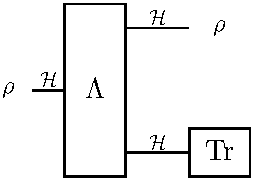
\includegraphics[scale=0.8]{broadcasting2.t1.pdf}
\end{minipage}
\begin{minipage}[c]{0.4\textwidth}
\centering
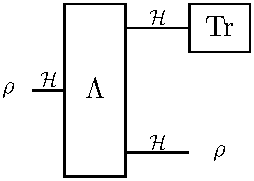
\includegraphics[scale=0.8]{broadcasting1.t1.pdf}
\end{minipage}
\end{center}

\medskip

 \structure{No-broadcasting}: for $\Lambda_1:=\mathrm {Tr}_2\circ\Lambda$,
 $\Lambda_2:=\mathrm {Tr}_1\circ\Lambda$,
\[
\Lambda_1(\rho)=\Lambda_2(\rho)=\rho \text{ for all }\rho 
 \text{ is \structure{impossible}}
 \]
  Restricted to  a subset $\Se$ of states:
\[
\text{Broadcasting is 
possible}\iff \Se  \text{ is
\structure{commutative}.}
\]



\end{frame}

\begin{frame}{Broadcasting and distinguishability}

Let $\rho,\sigma$ be states. Instead of broadcasting $\{\rho,\sigma\}$, we require
\bigskip

Both $\Lambda_1$ and $\Lambda_2$ preserve distinguishability of  $\rho,\sigma$:
\begin{align*}
P_e(\lambda,\Lambda_1(\rho),\Lambda_1(\sigma))&=P_e(\lambda,\Lambda_2(\rho),\Lambda_2(\sigma))\\[2mm]
&=P_e(\lambda,\rho,\sigma), \qquad  \ \lambda\in [0,1].
\end{align*}

\medskip

Then $\Lambda_1$, $\Lambda_2$ are reversible with respect to $\{\rho,\sigma\}$. If
$\Psi_1$, $\Psi_2$ are the recovery channels, then
\[
(\Psi_1\otimes \Psi_2)\circ \Lambda
\]
is a broadcasting channel for $\{\rho,\sigma\}$. Hence $\rho,\sigma$ must commute.




\end{frame}


\begin{frame}{Broadcasting and distinguishability}

If we assume $P_e(\lambda,\Lambda_1(\rho),\Lambda_1(\sigma))=P_e(\lambda,\rho,\sigma)$,
$\lambda\in [0,1]$:
\medskip

\begin{itemize}
\item there is a channel $\Lambda':B(\Ha)\to B(\Ha\otimes \Ha)$ such that
$\Lambda_1'$ preserves $\rho$ and $\sigma$ and
$(\Lambda'_1)^*$
is a conditional expectation, while  $\Lambda'_2=\Lambda_2$.

\item The ranges of $(\Lambda_1')^*$ and $\Lambda_2^*$ must commute
\item Any test on the second part acts on the commutant $\Me_{\{\rho,\sigma\}}'$
\item $P_e(\lambda,\Lambda_2(\rho),\Lambda_2(\sigma))\ge P_e(\lambda,
\mu(\rho),\mu(\sigma))$, $\lambda\in [0,1]$,
\vskip 3mm
 $\{\mu(\rho),\mu(\sigma)\}$ - the \structure{classical part} of the
Koashi-Imoto decomposition of $\{\rho,\sigma\}$.
\end{itemize}


\end{frame}

\end{document}


Put  $\Se=\{\rho,\sigma\}$ and  require that for all $\lambda\in [0,1]$,
\begin{align*}
P_e(\lambda,\Lambda_1(\rho),\mathrm{Tr}_1\circ\Lambda(\sigma))&=P_e(\lambda,\mathrm{Tr}_2\circ\Lambda(\rho),\mathrm{Tr}_2\circ\Lambda(\sigma))\\[2mm]
&=P_e(\lambda,\rho,\sigma).
\end{align*}


\medskip

\begin{itemize}
\item possible only if $\rho$ and $\sigma$ commute
\vskip 3mm

\item If $P_e(\lambda,\mathrm{Tr}_2\circ\Lambda(\rho),\mathrm{Tr}_2\circ\Lambda(\sigma))
=P_e(\lambda,\rho,\sigma)$ for all $\lambda$, then 
\[
P_e(\lambda,\mathrm{Tr}_1\circ\Lambda(\rho),\mathrm{Tr}_1\circ\Lambda(\sigma))\ge
P_e(\lambda, p,q),\quad \forall \lambda\in [0,1],
\]
$\{p,q\}$ is the classical part of $\{\rho,\sigma\}$.

\end{itemize}




\end{frame}



\end{document}
§
